\section{Fixed-direction controls at equal numerical budget}
Equal total L2 does not match temporal structure. We supplement the original random block interventions with fixed directions in each non-null block, using the same twenty saved cohorts, crop lengths, masks, normalization, reader weights and reference embeddings. Both signs and both radii are retained, without captions, gradients or score-selected directions.

For positions and velocities, the local unit direction $(1,1,1)/\sqrt3$ is repeated across joints and valid frames in unnormalized coordinates. Contacts use four equal entries. Rotations are right-multiplied by a local SO(3) change around the same signed axis, with a per-clip angle solved from the input norm and bounded by $\pi/2$. The directions are constant in time; the remaining blocks are protected. This is temporal coherence of the intervention, not consistency of an entire motion-feature vector. In particular, position changes do not update velocities, and rotation changes do not update positions. Continuous contact offsets can leave their binary domain; Guo does not consume that block.

The norm remains $\|D_r^{-1}(y-x)\|_2=\kappa\sqrt L$ per clip, before feature selection. Float32 contact offsets have coarser relative quantization on binary values: their realized norm tolerance is $2\times10^{-5}$, versus $5\times10^{-6}$ elsewhere. These limits concern relative input-norm error, not evaluator scores. The chosen directions and both budgets are fixed independently of the metric.

\begin{table*}[t]
\centering\small
\caption{\textbf{T2M fixed directions, all twenty draws.} Both signs and radii; paired $t_{19}$ intervals adjust 32 endpoints in this primary family. Directions are fixed in time, but held-fixed feature blocks may be physically inconsistent. T2M excludes contacts; TMR reads all 263 channels.}\label{tab:table_coherent_guo_fixed}
\begin{tabular}{@{}llrrrr@{}}\toprule
$\kappa$&Intervention&$\Delta$ FID&95\% interval&$\Delta$ R1 (pp)&95\% interval\\\midrule
1&Rotations $+$&+0.00086&$[+0.00086,+0.00087]$&-0.038&$[-0.186,+0.110]$\\
1&Rotations $-$&+0.00102&$[+0.00102,+0.00103]$&+0.064&$[-0.106,+0.233]$\\
1&Velocities $+$&+0.00790&$[+0.00787,+0.00793]$&-0.073&$[-0.280,+0.133]$\\
1&Velocities $-$&+0.01773&$[+0.01767,+0.01779]$&-0.071&$[-0.257,+0.115]$\\
1&Contacts $+$&+0.00000&$[-0.00000,+0.00000]$&+0.000&$[+0.000,+0.000]$\\
1&Contacts $-$&+0.00000&$[-0.00000,+0.00000]$&+0.000&$[+0.000,+0.000]$\\
1&Positions $+$&+0.02842&$[+0.02832,+0.02852]$&+0.147&$[-0.061,+0.354]$\\
1&Positions $-$&+0.04435&$[+0.04424,+0.04447]$&-0.312&$[-0.566,-0.059]$\\
3&Rotations $+$&+0.01061&$[+0.01056,+0.01066]$&-0.184&$[-0.467,+0.099]$\\
3&Rotations $-$&+0.01512&$[+0.01507,+0.01517]$&+0.165&$[-0.057,+0.386]$\\
3&Velocities $+$&+0.06033&$[+0.06020,+0.06046]$&-0.247&$[-0.577,+0.083]$\\
3&Velocities $-$&+0.47604&$[+0.47496,+0.47712]$&-0.945&$[-1.293,-0.597]$\\
3&Contacts $+$&+0.00000&$[-0.00000,+0.00000]$&+0.000&$[+0.000,+0.000]$\\
3&Contacts $-$&+0.00000&$[-0.00000,+0.00000]$&+0.000&$[+0.000,+0.000]$\\
3&Positions $+$&+0.34160&$[+0.34071,+0.34249]$&-0.700&$[-1.107,-0.294]$\\
3&Positions $-$&+1.18896&$[+1.18691,+1.19101]$&-2.524&$[-2.917,-2.131]$\\
\bottomrule\end{tabular}\end{table*}

\begin{table*}[t]
\centering\small
\caption{\textbf{TMR fixed directions, all twenty draws.} Both signs and radii; paired $t_{19}$ intervals adjust 32 endpoints in this primary family. Directions are fixed in time, but held-fixed feature blocks may be physically inconsistent. Guo excludes contacts; TMR reads all 263 channels.}\label{tab:table_coherent_tmr_fixed}
\begin{tabular}{@{}llrrrr@{}}\toprule
$\kappa$&Intervention&$\Delta$ cosine&95\% interval&$\Delta$ R1 (pp)&95\% interval\\\midrule
1&Rotations $+$&-0.00048&$[-0.00052,-0.00045]$&-0.015&$[-0.094,+0.064]$\\
1&Rotations $-$&-0.00005&$[-0.00008,-0.00001]$&+0.015&$[-0.073,+0.103]$\\
1&Velocities $+$&-0.00074&$[-0.00078,-0.00070]$&+0.005&$[-0.083,+0.094]$\\
1&Velocities $-$&-0.00020&$[-0.00024,-0.00016]$&-0.036&$[-0.130,+0.059]$\\
1&Contacts $+$&-0.00034&$[-0.00047,-0.00021]$&+0.061&$[-0.140,+0.263]$\\
1&Contacts $-$&-0.00605&$[-0.00620,-0.00590]$&-0.353&$[-0.529,-0.178]$\\
1&Positions $+$&-0.00019&$[-0.00024,-0.00014]$&-0.036&$[-0.137,+0.066]$\\
1&Positions $-$&-0.00081&$[-0.00085,-0.00076]$&-0.012&$[-0.105,+0.081]$\\
3&Rotations $+$&-0.00319&$[-0.00331,-0.00308]$&-0.217&$[-0.355,-0.079]$\\
3&Rotations $-$&-0.00173&$[-0.00183,-0.00163]$&+0.009&$[-0.179,+0.196]$\\
3&Velocities $+$&-0.00522&$[-0.00535,-0.00508]$&-0.224&$[-0.421,-0.028]$\\
3&Velocities $-$&-0.00378&$[-0.00392,-0.00364]$&-0.186&$[-0.366,-0.007]$\\
3&Contacts $+$&-0.01998&$[-0.02030,-0.01966]$&-0.835&$[-1.163,-0.507]$\\
3&Contacts $-$&-0.04677&$[-0.04726,-0.04629]$&-2.316&$[-2.640,-1.991]$\\
3&Positions $+$&-0.00375&$[-0.00392,-0.00359]$&-0.175&$[-0.300,-0.049]$\\
3&Positions $-$&-0.00552&$[-0.00564,-0.00540]$&-0.081&$[-0.215,+0.053]$\\
\bottomrule\end{tabular}\end{table*}

\begin{table*}[t]
\centering\small
\caption{\textbf{T2M fixed minus random, all twenty draws.} Both signs and radii; paired $t_{19}$ intervals adjust 32 endpoints in this secondary contrast family. Directions are fixed in time, but held-fixed feature blocks may be physically inconsistent. T2M excludes contacts; TMR reads all 263 channels.}\label{tab:table_coherent_guo_contrast}
\begin{tabular}{@{}llrrrr@{}}\toprule
$\kappa$&Intervention&$\Delta$ FID&95\% interval&$\Delta$ R1 (pp)&95\% interval\\\midrule
1&Rotations $+$&+0.00080&$[+0.00080,+0.00081]$&-0.059&$[-0.216,+0.098]$\\
1&Rotations $-$&+0.00096&$[+0.00096,+0.00097]$&+0.042&$[-0.123,+0.207]$\\
1&Velocities $+$&+0.00772&$[+0.00770,+0.00775]$&-0.096&$[-0.263,+0.071]$\\
1&Velocities $-$&+0.01755&$[+0.01749,+0.01761]$&-0.094&$[-0.303,+0.116]$\\
1&Contacts $+$&+0.00000&$[-0.00000,+0.00000]$&+0.000&$[+0.000,+0.000]$\\
1&Contacts $-$&+0.00000&$[-0.00000,+0.00000]$&+0.000&$[+0.000,+0.000]$\\
1&Positions $+$&+0.02821&$[+0.02810,+0.02831]$&+0.098&$[-0.136,+0.332]$\\
1&Positions $-$&+0.04414&$[+0.04402,+0.04425]$&-0.361&$[-0.586,-0.136]$\\
3&Rotations $+$&+0.00712&$[+0.00704,+0.00719]$&-0.221&$[-0.499,+0.057]$\\
3&Rotations $-$&+0.01162&$[+0.01154,+0.01170]$&+0.128&$[-0.081,+0.337]$\\
3&Velocities $+$&+0.04447&$[+0.04423,+0.04471]$&-0.224&$[-0.484,+0.036]$\\
3&Velocities $-$&+0.46018&$[+0.45917,+0.46120]$&-0.922&$[-1.239,-0.606]$\\
3&Contacts $+$&+0.00000&$[-0.00000,+0.00000]$&+0.000&$[+0.000,+0.000]$\\
3&Contacts $-$&+0.00000&$[-0.00000,+0.00000]$&+0.000&$[+0.000,+0.000]$\\
3&Positions $+$&+0.32334&$[+0.32225,+0.32443]$&-0.671&$[-1.008,-0.335]$\\
3&Positions $-$&+1.17070&$[+1.16865,+1.17274]$&-2.495&$[-2.863,-2.126]$\\
\bottomrule\end{tabular}\end{table*}

\begin{table*}[t]
\centering\small
\caption{\textbf{TMR fixed minus random, all twenty draws.} Both signs and radii; paired $t_{19}$ intervals adjust 32 endpoints in this secondary contrast family. Directions are fixed in time, but held-fixed feature blocks may be physically inconsistent. Guo excludes contacts; TMR reads all 263 channels.}\label{tab:table_coherent_tmr_contrast}
\begin{tabular}{@{}llrrrr@{}}\toprule
$\kappa$&Intervention&$\Delta$ cosine&95\% interval&$\Delta$ R1 (pp)&95\% interval\\\midrule
1&Rotations $+$&-0.00059&$[-0.00063,-0.00054]$&-0.027&$[-0.108,+0.054]$\\
1&Rotations $-$&-0.00015&$[-0.00018,-0.00011]$&+0.003&$[-0.094,+0.101]$\\
1&Velocities $+$&-0.00076&$[-0.00080,-0.00072]$&+0.006&$[-0.118,+0.131]$\\
1&Velocities $-$&-0.00022&$[-0.00027,-0.00017]$&-0.034&$[-0.131,+0.062]$\\
1&Contacts $+$&-0.00042&$[-0.00056,-0.00027]$&+0.060&$[-0.133,+0.253]$\\
1&Contacts $-$&-0.00612&$[-0.00627,-0.00598]$&-0.355&$[-0.544,-0.165]$\\
1&Positions $+$&-0.00028&$[-0.00034,-0.00023]$&-0.054&$[-0.166,+0.058]$\\
1&Positions $-$&-0.00090&$[-0.00096,-0.00085]$&-0.030&$[-0.145,+0.084]$\\
3&Rotations $+$&-0.00404&$[-0.00418,-0.00391]$&-0.239&$[-0.373,-0.105]$\\
3&Rotations $-$&-0.00258&$[-0.00268,-0.00248]$&-0.014&$[-0.206,+0.178]$\\
3&Velocities $+$&-0.00525&$[-0.00538,-0.00512]$&-0.223&$[-0.412,-0.034]$\\
3&Velocities $-$&-0.00382&$[-0.00398,-0.00365]$&-0.185&$[-0.344,-0.027]$\\
3&Contacts $+$&-0.01876&$[-0.01912,-0.01840]$&-0.600&$[-0.844,-0.356]$\\
3&Contacts $-$&-0.04555&$[-0.04598,-0.04513]$&-2.081&$[-2.344,-1.818]$\\
3&Positions $+$&-0.00445&$[-0.00464,-0.00426]$&-0.205&$[-0.361,-0.048]$\\
3&Positions $-$&-0.00622&$[-0.00640,-0.00605]$&-0.111&$[-0.274,+0.052]$\\
\bottomrule\end{tabular}\end{table*}


Each reader's primary family contains 32 endpoints: four blocks, two signs, two radii and two scores. Separate secondary 32-endpoint families compare each fixed intervention with its original random block control on the same cohorts. Paired $t_{19}$ intervals use Bonferroni adjustment within each family. The historical null/random family remains 28 endpoints; the two phases are not presented as one prospective test. Matched-reference real-data FID starts at zero by construction. Numerically negligible nonzero contact FID can arise in the distance computation despite bitwise-identical Guo embeddings.

All metric cells, primary intervals and fixed-minus-random contrasts are recomputed independently. Every saved per-clip norm is checked, and the first eight fixtures per condition/draw are reconstructed using separate formulas and SciPy rotations. Native forward checks verify the saved embeddings, including Guo's caption/length reordering. Protected channels and padding are compared bitwise; the non-null rotation controls must change represented matrices. These checks do not claim complete geometry replay of unsaved arrays.

\begin{figure*}[t]\centering
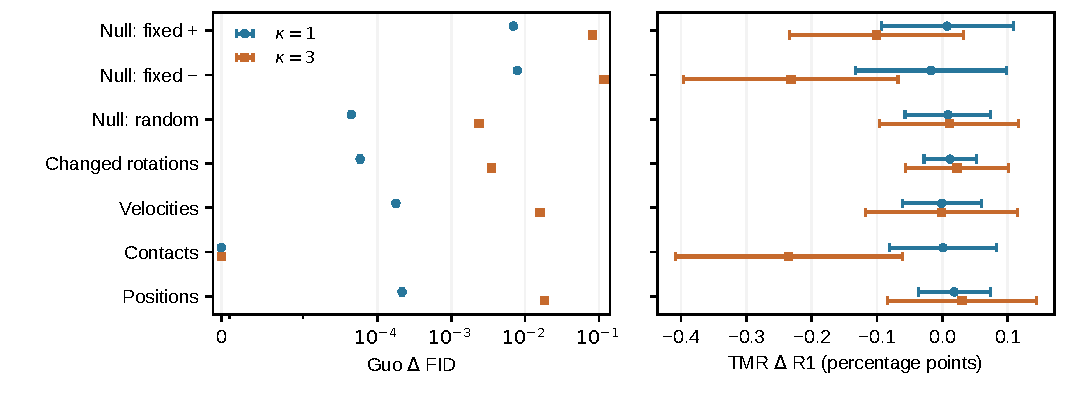
\includegraphics[width=\textwidth]{figures/matched_blocks_random.pdf}
\caption{\textbf{The original random/null controls, both radii.} All twenty draws; the historical 28-endpoint intervals remain unchanged. Here $\kappa$ denotes the numerical budget and $\rho$ remains the positive scale in the rotation fiber. Random position/velocity noise has a larger Guo FID effect than random fiber coefficients at the larger budget. This plot is distinct from the additional fixed-direction controls in the main paper.}\label{fig:randomblocks}
\end{figure*}

\section{Real sign inputs without an attack}
\begin{table*}[t]
\centering\small
\caption{\textbf{Natural dependence in real sign inputs, no attack.} Full native test with common loader preprocessing and frozen raw reader; no source-conditioned layer, optimization or new decoding. The shared left-hand preprocessing precedes both paths. Hypothesis counts and six BLEUs are independently recomputed; the CSL score is character-level.}\label{tab:signnatural}
\begin{tabular}{@{}llrrrr@{}}\toprule
Corpus&Changed / clips&Changed \%&Raw BLEU&$\C$ BLEU&$\C-$raw\\\midrule
PHOENIX&0/642&0.0\%&14.9995&14.9995&+0.0000\\
How2Sign&1,438/2,183&65.9\%&3.4779&3.4840&+0.0062\\
CSL-Daily&464/1,162&39.9\%&6.8907&7.0662&+0.1755\\
\bottomrule\end{tabular}\end{table*}

The same frozen raw reader decodes each real input and its canonical representative. There is no learned layer, source-caption conditioning, per-clip optimization or new model fitting. The restored results use the saved full native TEST hypotheses rather than a newly selected subset. Both paths share the original native preprocessing, including projection of left-hand channels 60:150 before decoding. Thus ``raw'' denotes the audit input under that shared preprocessing, not untouched bytes of the public release.

Independent code compares all 3,987 pairs of saved strings and recalculates the six corpus BLEUs from clipped n-gram counts and brevity penalties. PHOENIX changes 0/642 hypotheses; How2Sign changes 1,438/2,183; CSL changes 464/1,162. Scores use word tokens for PHOENIX/How2Sign and characters with punctuation retained for CSL. The full changed fractions are 0\%, 65.9\% and 39.9\%. Small corpus-score differences do not imply sentence-level invariance, improved semantics or an accuracy-free defense. Reader adaptation on noncanonical inputs is reported separately.
